\chapter{Architecture of the application}\label{sect:architecture}

\section {Spring Framework}
\tab Spring Framework \cite{spring_in_action} is a Java framework that supports the development of Java applications by providing complete infrastructure support. Spring takes care of the infrastructure, allowing you to concentrate on your application.

\tab Spring allows you to create apps out of "plain old Java objects" (POJOs) and non-invasively deploy corporate services to POJOs. This feature applies to both complete and partial Java EE as well as the Java SE programming model.

As an application framework, here are some examples of how you can take advantage of the Spring platform:
\begin{itemize}
    \item Without having to deal with transaction APIs, you may make a Java method execute in a database transaction.
    \item Without having to deal with remote APIs, you can turn a local Java method into a remote procedure.
    \item Without having to interact with JMX APIs, you can turn a local Java method into a management activity.
    \item Without having to deal with JMS APIs, you can turn a local Java method into a message handler.
\end{itemize}

\subsection*{Modules}
\tab The Spring Framework is made up of around 20 modules, each with its own set of functionality. As indicated in the figure, these modules are divided into Core Container, Data Access/Integration, Web, AOP (Aspect Oriented Programming), Instrumentation, and Test. \newline

\begin{center}
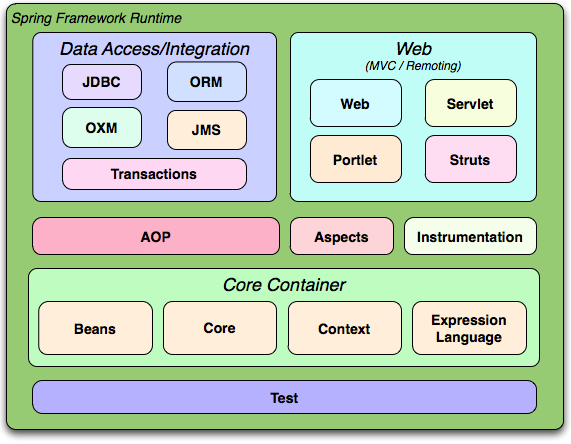
\includegraphics[width=300pt]{spring modules.PNG} 
\newline Overview of the Spring Framework
\end{center}

\section {Database scheme}
\tab Details about Database scheme ...
\newline

\section {Architecture of the application}
\tab Details about Architecture of the application ... \newline
\tab Maybe use micro-services ??? 
